%!TEX root = ./cikm2016.tex

%\section{Related Work}
\smallhead{Related work}
The literature on data factorisation and vector space models for
relational data is vast.
%or low-rank approximation is vast.
We give a brief overview of related work along three design choices:
%with respect to three orthogonal dimensions,
the method, the learning strategy, and the data representation.
%We then use these dimensions to help position our work.
%\item[Statistical method] With an statistical assumption used to develop
%underlying model structure, we broadly categorise models into Bayesian
%and non-Bayesian models.
In Table \ref{tbl:relatedwork}, we summarise related work along all combinations in each dimension.
Our work address the uncovered combination of three design choices in the probabilistic method, indicated by an asterisk.

\smallhead{Probabilistic (Pr) / Non-Probabilistic (N-Pr)} This refers to two broad classes of model
formulation, whether an obtained model has a probabilistic interpretation.
%The probabilistic models are capable of placing priors and measuring uncertainty.

\smallhead{Passive (P) / Active (A)} This refers to two different learning strategies,
of passively learning a model given labeled data points, or actively
requesting data points to be labelled.

\smallhead{Matrix (M) / Tensor (T) / Composition (C)} This refers to three data representations. Matrix represents single relational data such as \texttt{(user, item)}.
% Matrix representation of data is common when a dataset can be represented as a bi-partite graph, such as (user, item).
Tensor represents multiple relational data such as \texttt{(entity, relation, entity2)}.
%Tensor representation is handy when edges in the graph have labels, i.e. (entity1, relation, entity2).
Composition includes more complex structures of multiple relational data such as \texttt{(entity1 -- relation1 -- entity2 -- relation2 -- entity3)}. 

Model details and additional results can be found in the online appendix~\cite{kim2016probabilistic}. 
%An extended version of this paper is at \url{http://cm.cecs.anu.edu.au/documents/prescal_appendix.pdf}.
%We can think of compositions as paths in the graph, i.e. (entity1 -- relation1 -- entity2 -- relation2 -- entity3).


%Note that N-Pr, A, C, or Non-Probabilistic Active Composition model, can be done by
%simply using the query strategies from \cite{kajino2015active} on the
%compositional model by \cite{guu2015traversing}.
% a critical gap
%in Probabilistic tensor factorisation (Pr) capable of Active learning (A) with Compositions of  relations (C).
\eat{The knowledge graph construction has been widely focused in the natural
language processing communities.
Manual data acquisition with human crafted
or automatically inferred synthetic rules or distant supervision on a large
amount of unlabelled text are the main tools to construct \cite{fader2011identifying,Mintz2009}.}

\eat{
Given this position, our work is inspired by, and most closely related to:
active multi-relational data construction (AMDC)
with tensor factorisation~\cite{kajino2015active},
Thomson sampling for matrix factorisation~\cite{kawale2015efficient},
and compositional objectives in vector space~\cite{guu2015traversing}.
Note that we reformulate the compositional objectives probabilistically such that it can be used in an active setting;
our approach for active learning is a generalisation of
Thomson sampling from matrixes to tensors;
AMDC find that reconstruction accuracy and knowledge population
cannot be achieved at the same time with strategies geared towards
either exploit or reducing uncertainty,
we show that the two objectives can be achieved at the same time with
a properly designed exploration-exploitation scheme.
}
\eat{show active knowledge graph construction
algorithm based on the low-rank structure. They proposed active
multi-relational data construction (AMDC) with two separate problems:
a knowledge base population and predictive model construction, and show
that these two goals cannot be achieved at the same time. In this work,
we show that it can be achieved at the same time with a properly designed
exploration and exploitation scheme that has been shown in the matrix
factorisation problem \cite{kawale2015efficient}.
}


%\begin{itemize}
%\item [B,A,M] Efficient Thompson Sampling for OnlineMatrix-Factorization Recommendation\cite{kawale2015efficient}. Active learning and search on low-rank matrices \cite{sutherland2013active}. Collaborative filtering as multi armed bandit \cite{guillou2015collaborative}
%\item [N,A,M] Matrix completion with queries \cite{ruchansky2015matrix}.
%\item [B,P,M] PMF \cite{mnih2007probabilistic} ...
%\item [N,P,M] NMF\cite{lee1999learning} ...
%\item [B,P,T] Bayesian Tensor Factorisation models. CANDECOMP/PARAFAC (CP) decomposition \cite{xiong2010temporal,schmidt2009probabilistic}, CP and TUCKER3 \cite{yilmaz2012algorithms}
%\item [N,A,T] Populating knowledge graph with active learning (IBM) \cite{kajino2015active}
%\item [N,P,T] Rescal \cite{nickel2011three}, TransE \cite{bordes2013translating}, and many others.
%\item [N,P,C] Compositional vector space model \cite{Neelakantan2015},
%\end{itemize}
%
%Might be relevant, but not positioned in the figure.
%\begin{itemize}
%\item Clustering based Bayesian approach for learning relations: Infinite relational model based on entity clustering \cite{kemp2006learning}.
%\item Path ranking algorithm (graph feature model) \cite{Lao2010}
%\end{itemize}

%\begin{figure}[t]
%	\centering
%	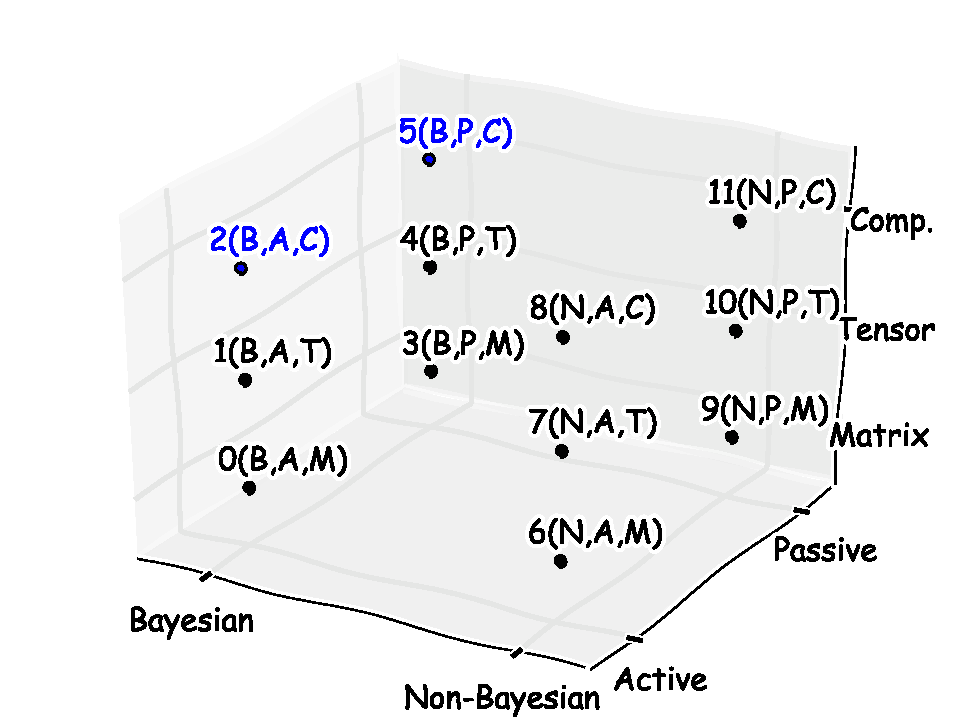
\includegraphics[width=\linewidth]{images/3d_plot.pdf}
%	\caption{\label{fig:related3d}Scope of our work}
%\end{figure}
